% TikZ 代码: 星形线 (astroid) - 参数方程 x=a*cos³θ, y=a*sin³θ
% 这是一个手动编写的测试样例
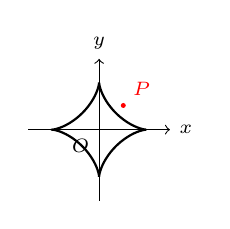
\begin{tikzpicture}[scale=0.6,baseline=-0.5ex]
  % 坐标轴
  \draw[->] (-1.5,0) -- (1.5,0) node[right] {\scriptsize $x$};
  \draw[->] (0,-1.5) -- (0,1.5) node[above] {\scriptsize $y$};
  
  % 星形线 (astroid): x = cos³θ, y = sin³θ (a=1 for simplicity)
  \draw[thick,smooth,samples=100,domain=0:360,variable=\t] 
    plot ({cos(\t)^3},{sin(\t)^3});
  
  % 标记点 P(x₀, y₀)
  \fill[red] (0.512,0.512) circle (1.5pt) node[above right] {\scriptsize $P$};
  
  % 原点
  \node[below left] at (0,0) {\scriptsize $O$};
\end{tikzpicture}